\section{Results and Discussion}

In this section, we report the findings of our user study that compare the proposed MindMargin interface against the traditional vertical commenting system. Overall, we observed a decrease in polarized views among readers who had seen or read the article previously and an increase in opinion polarization among unfamiliar readers. We also found an increase in readers' positive impressions of comments when using MindMargin. We were able to accept both of our hypotheses.

\subsection{Hypothesis 1}
Our first hypothesis predicted an impact on individual opinions: prompting new readers to develop a stance on an issue and encouraging readers with existing views to consider alternate views. The reasoning behind this hypothesis was that MindMargin exposes readers to a greater number of opinions while reading the article. Consequently, readers think more independently and sharpen their opinions. All participants were asked their stance, from Strongly For TFA to Strongly Against TFA, on a Likert scale. During analysis, we excluded data from participants who reported to have not read the comments (there was no difference in stance between prototypes there). We also excluded participants who did not toggle the Likert scale. The data of the remaining participants (N=XX) was remapped for their "stance extremeness" as $|50 - stance|$ (range 0-50). All participants reported on their familiarity with the article as choices of "none, seen or read". We then performed an analysis for both prototypes including this familiarity with the article as a covarying factor and the dependent variable "stance extremeness SE". We found that there was no significant difference in stance between MindMargin and the traditional commenting system when users did not know the article before. For participants who were familiar, we did observe a difference in individual stance between the prototypes (see figure YYYY). Participants who have seen this article before had a SE of 7 with MindMargin and 17 with the traditional system. Participants who have read this article before had a SE value of 17 with MindMargin and 27 with the traditional system. XXXXXX TODO: talk about p-value here and trend since not significant, also interpretation/discussion XXXXX. Unfortunately, we did not query the participants for their individual stance prior to showing the article which is a limitation of our experiment and will be addressed in future research.



\subsection{Hypothesis 2}
Our second hypothesis predicted an overall increase in positive impressions on comments when using the MindMargin interface. We asked participants who read the comments to input two adjectives in free-text describing either their reaction to the comments or a description of the comments. We then asked four independent volunteers to classify these adjectives using a four-bin classifier ("Positive", "Negative", "Neutral" and "Invalid"). We used the resulting mean encoding to classify the specified adjectives. Then, we compared the impressions between MindMargin and the traditional commenting system. We observed a drastic change of impressions when using MindMargin. As seen in figure \ref{fig:trad_pie}, the majority of participants using the traditional commenting system described the comments as negative (68\%). In contrast, when using MindMargin, the majority of participants described the comments as positive (48\%) or neutral (48\%) as seen in figure \ref{fig:mm_pie}. "Invalid" adjectives were also observed only to occur in the traditional commenting system. XXXX TODO: Ordinal regression? Discussion XXXX We have therefore \textbf{accepted Hypothesis~2}. 

\marginpar{
\begin{figure}
  \begin{center}
  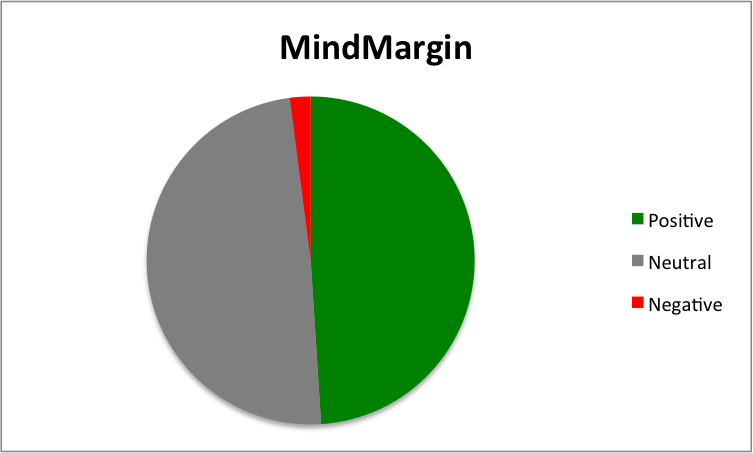
\includegraphics[width=\marginparwidth]{mm_piechart.png}
  \caption{When using MindMargin, the majority of participants described the comments as positive.}
  \label{fig:mm_pie}
  \end{center}
\end{figure}
}

\marginpar{
\begin{figure}
  \begin{center}
  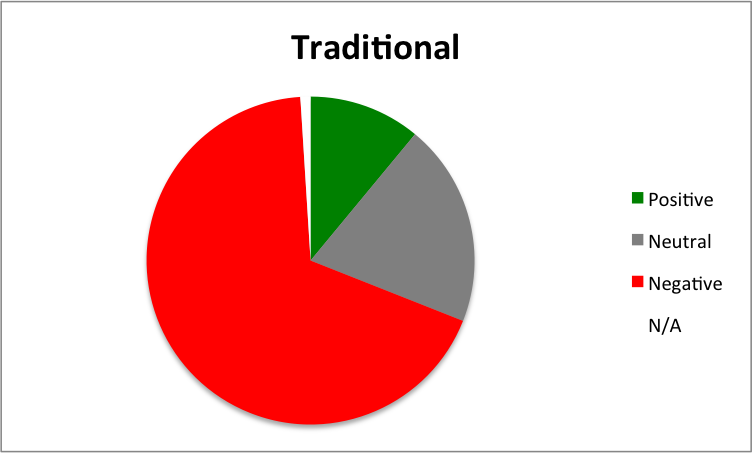
\includegraphics[width=\marginparwidth]{traditional_piechart.png}
  \caption{The majority of participants using the traditional commenting system described the comments as negative.}
  \label{fig:trad_pie}
  \end{center}
\end{figure}
}

In addition to our quantitative results, we would like to quote qualitative feedback from a MindMargin user, suggesting actions he/she took beyond the scope of reading and commenting article: "This article showed me a new perspective on TFA, which after doing research, I have realized I agree with." No feedback suggesting actions outside the scope of the article was received from participants with the traditional commenting system. 